    \begin{center}
        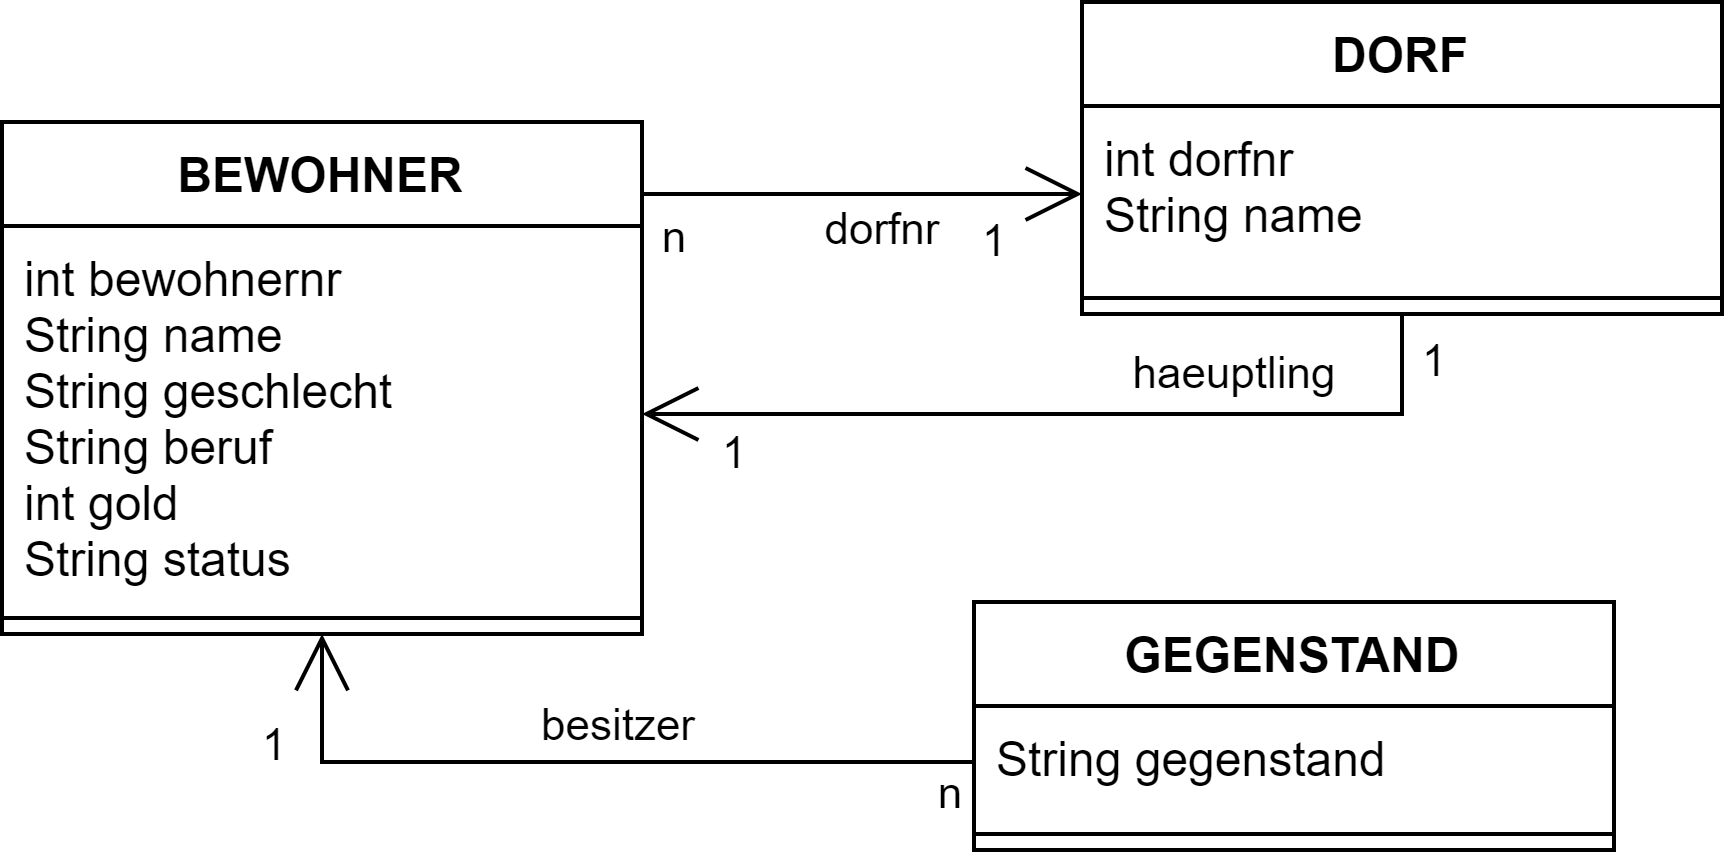
\includegraphics[width=.55\textwidth]{Aufgaben/SQL-DFD_Uebung_img/DB.png}
    \end{center}
     

    \section{SQL-Abfragen aus mehreren Tabellen}
    Zeichne für jede Aufgabe zuerst das Datenflussdiagramm und formuliere anschließend die SQL-Abfrage. Achte darauf, dass nicht mehr als gefragt ausgegeben wird.\\


    1. Gib die Name aller Bewohner aus.

    \LoesungKaro{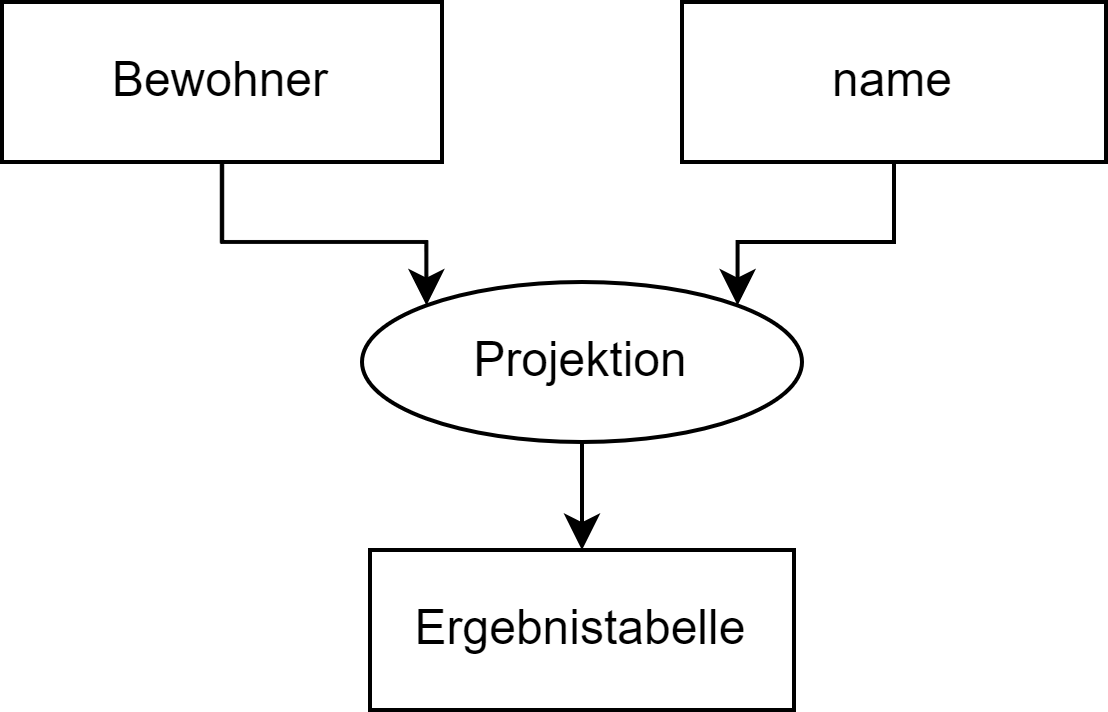
\includegraphics[width=0.4\textwidth]{Aufgaben/SQL-DFD_Uebung_img/1.png}}{9}

    \LoesungLine{SELECT name\\FROM Bewohner}{1}

    2. Gib die Daten aller Bewohner und des jeweiligen Heimatdorfs aus.

    \LoesungKaro{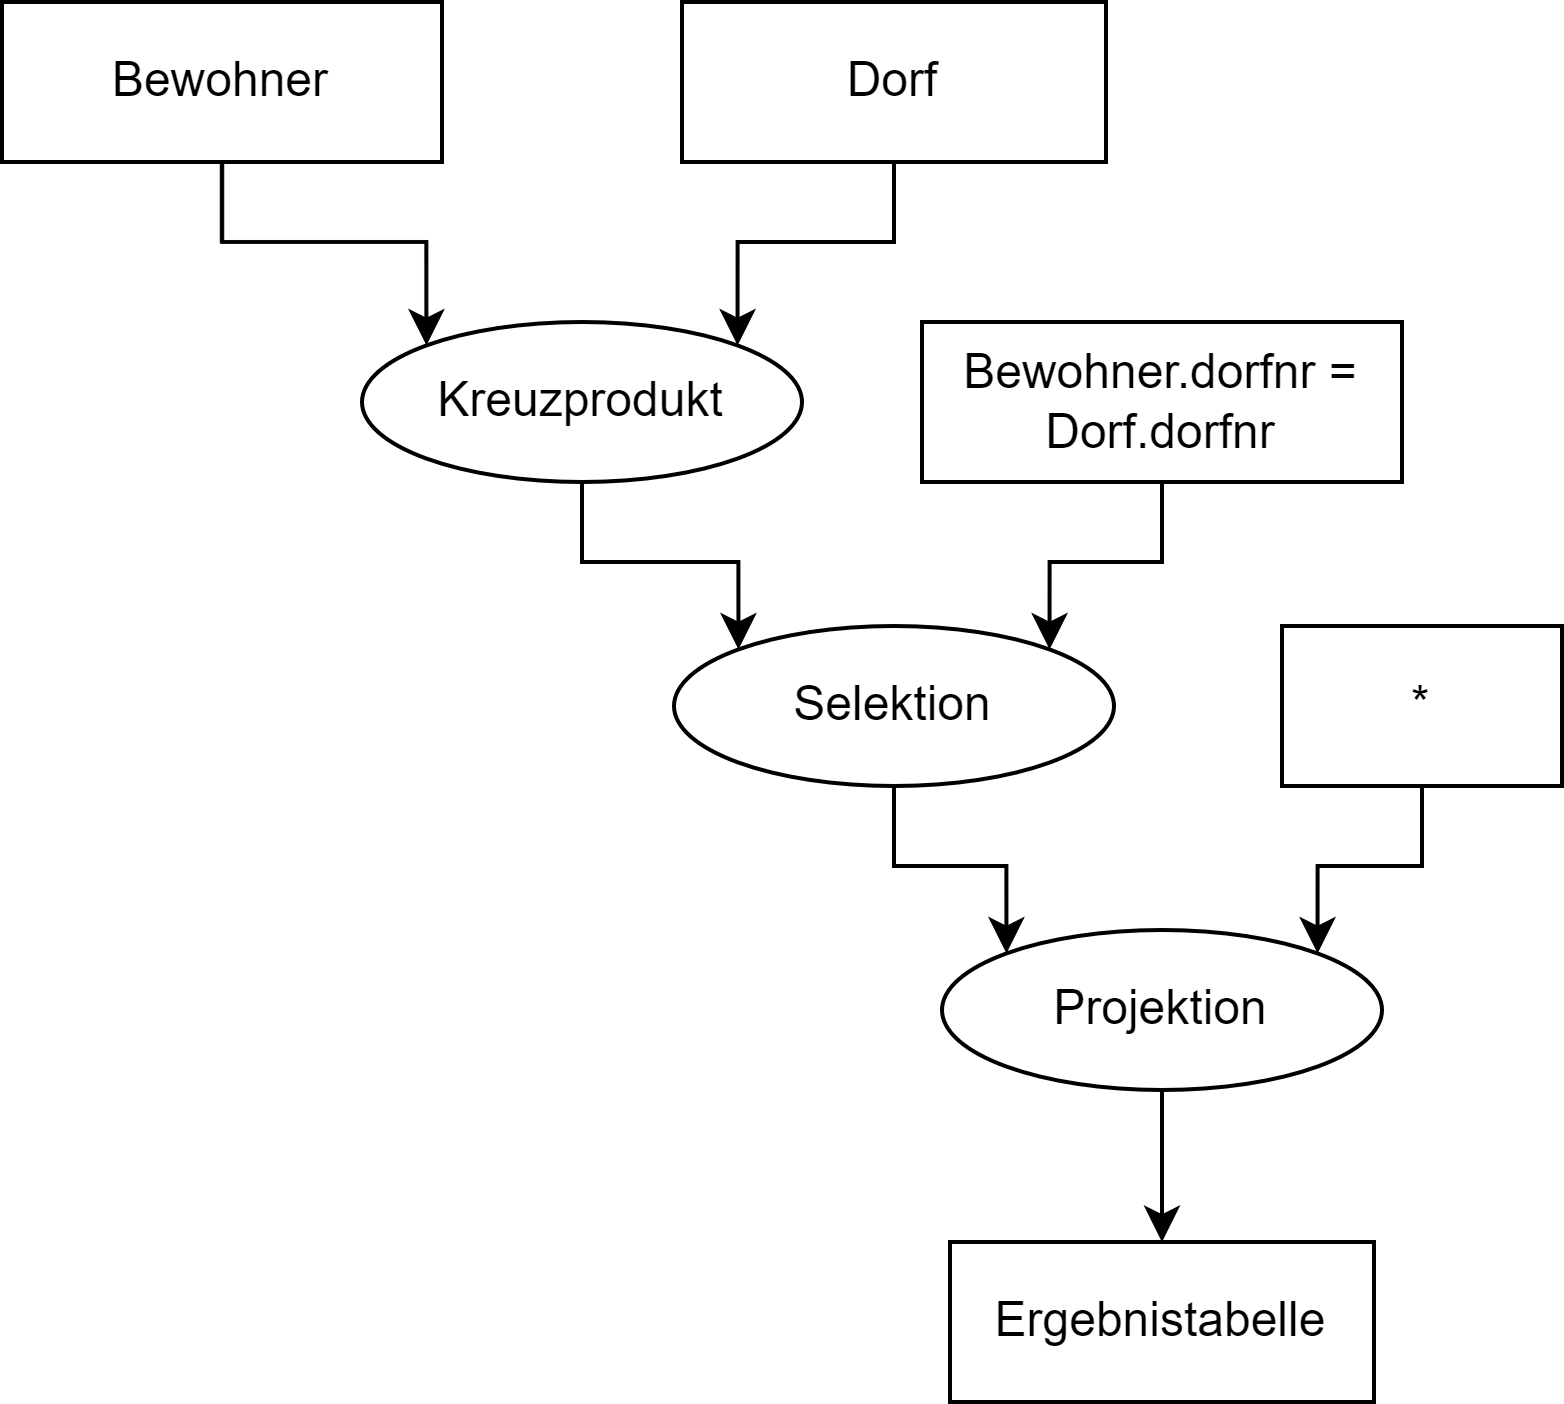
\includegraphics[width=0.6\textwidth]{Aufgaben/SQL-DFD_Uebung_img/2.png}}{15}

    \LoesungLine{SELECT * \\ FROM Bewohner, Dorf \\ WHERE bewohner.dorfnr=Dorf.dorfnr}{2}

    3. Gib die Bezeichner aller Gegenstände und den Namen ihrer Besitzer aus.

    \LoesungKaro{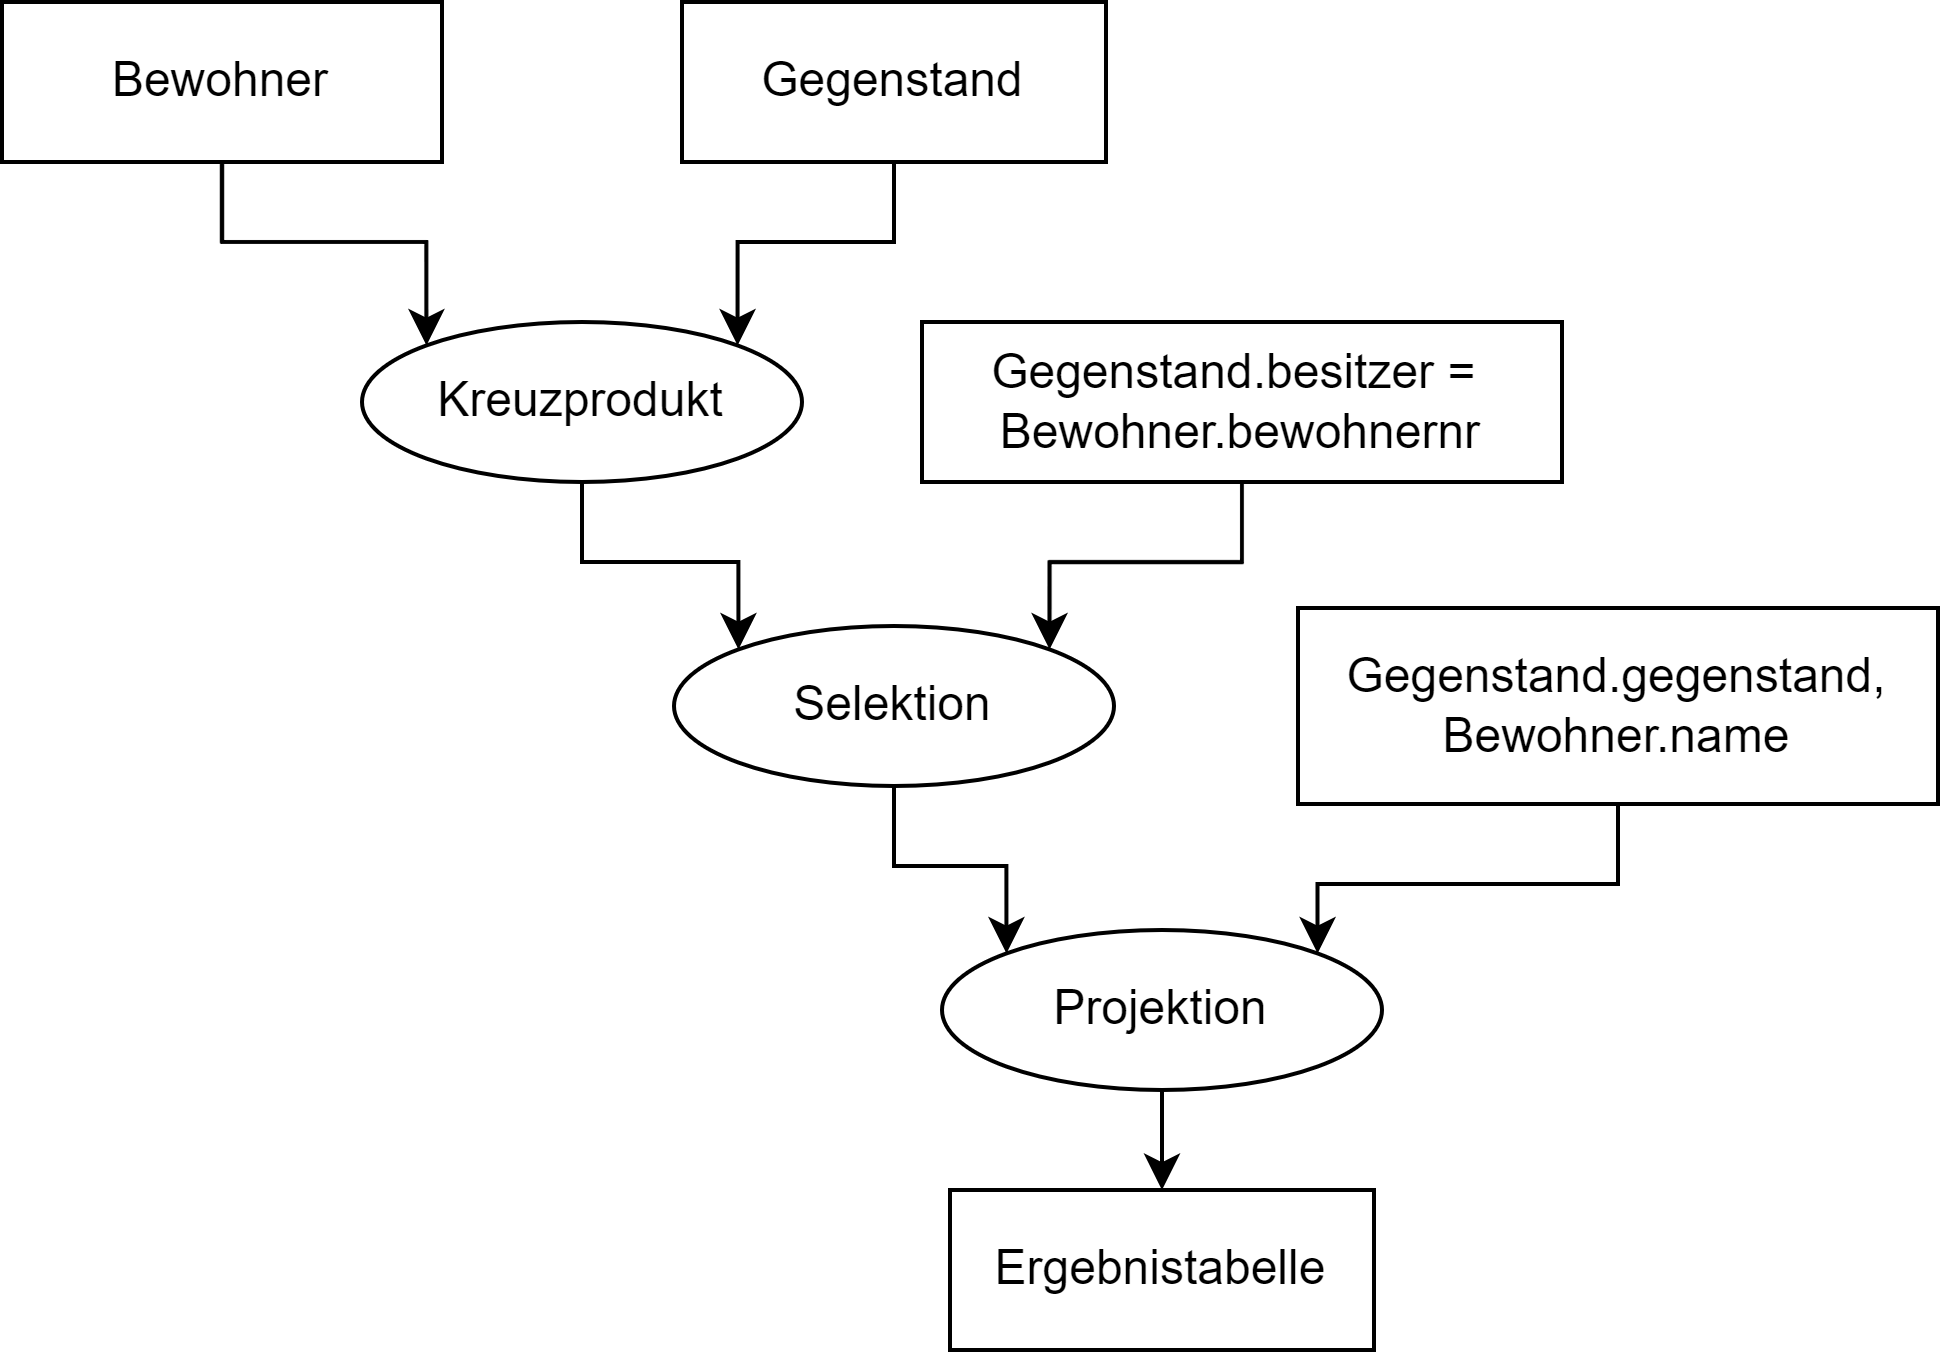
\includegraphics[width=0.8\textwidth]{Aufgaben/SQL-DFD_Uebung_img/3.png}}{17}

    \LoesungLine{SELECT gegenstand,name \\ FROM Gegenstand,Bewohner \\ WHERE besitzer=bewohnernr}{2}

    4. Gib die Daten aller Bewohner von Affenstadt aus.

    \LoesungKaro{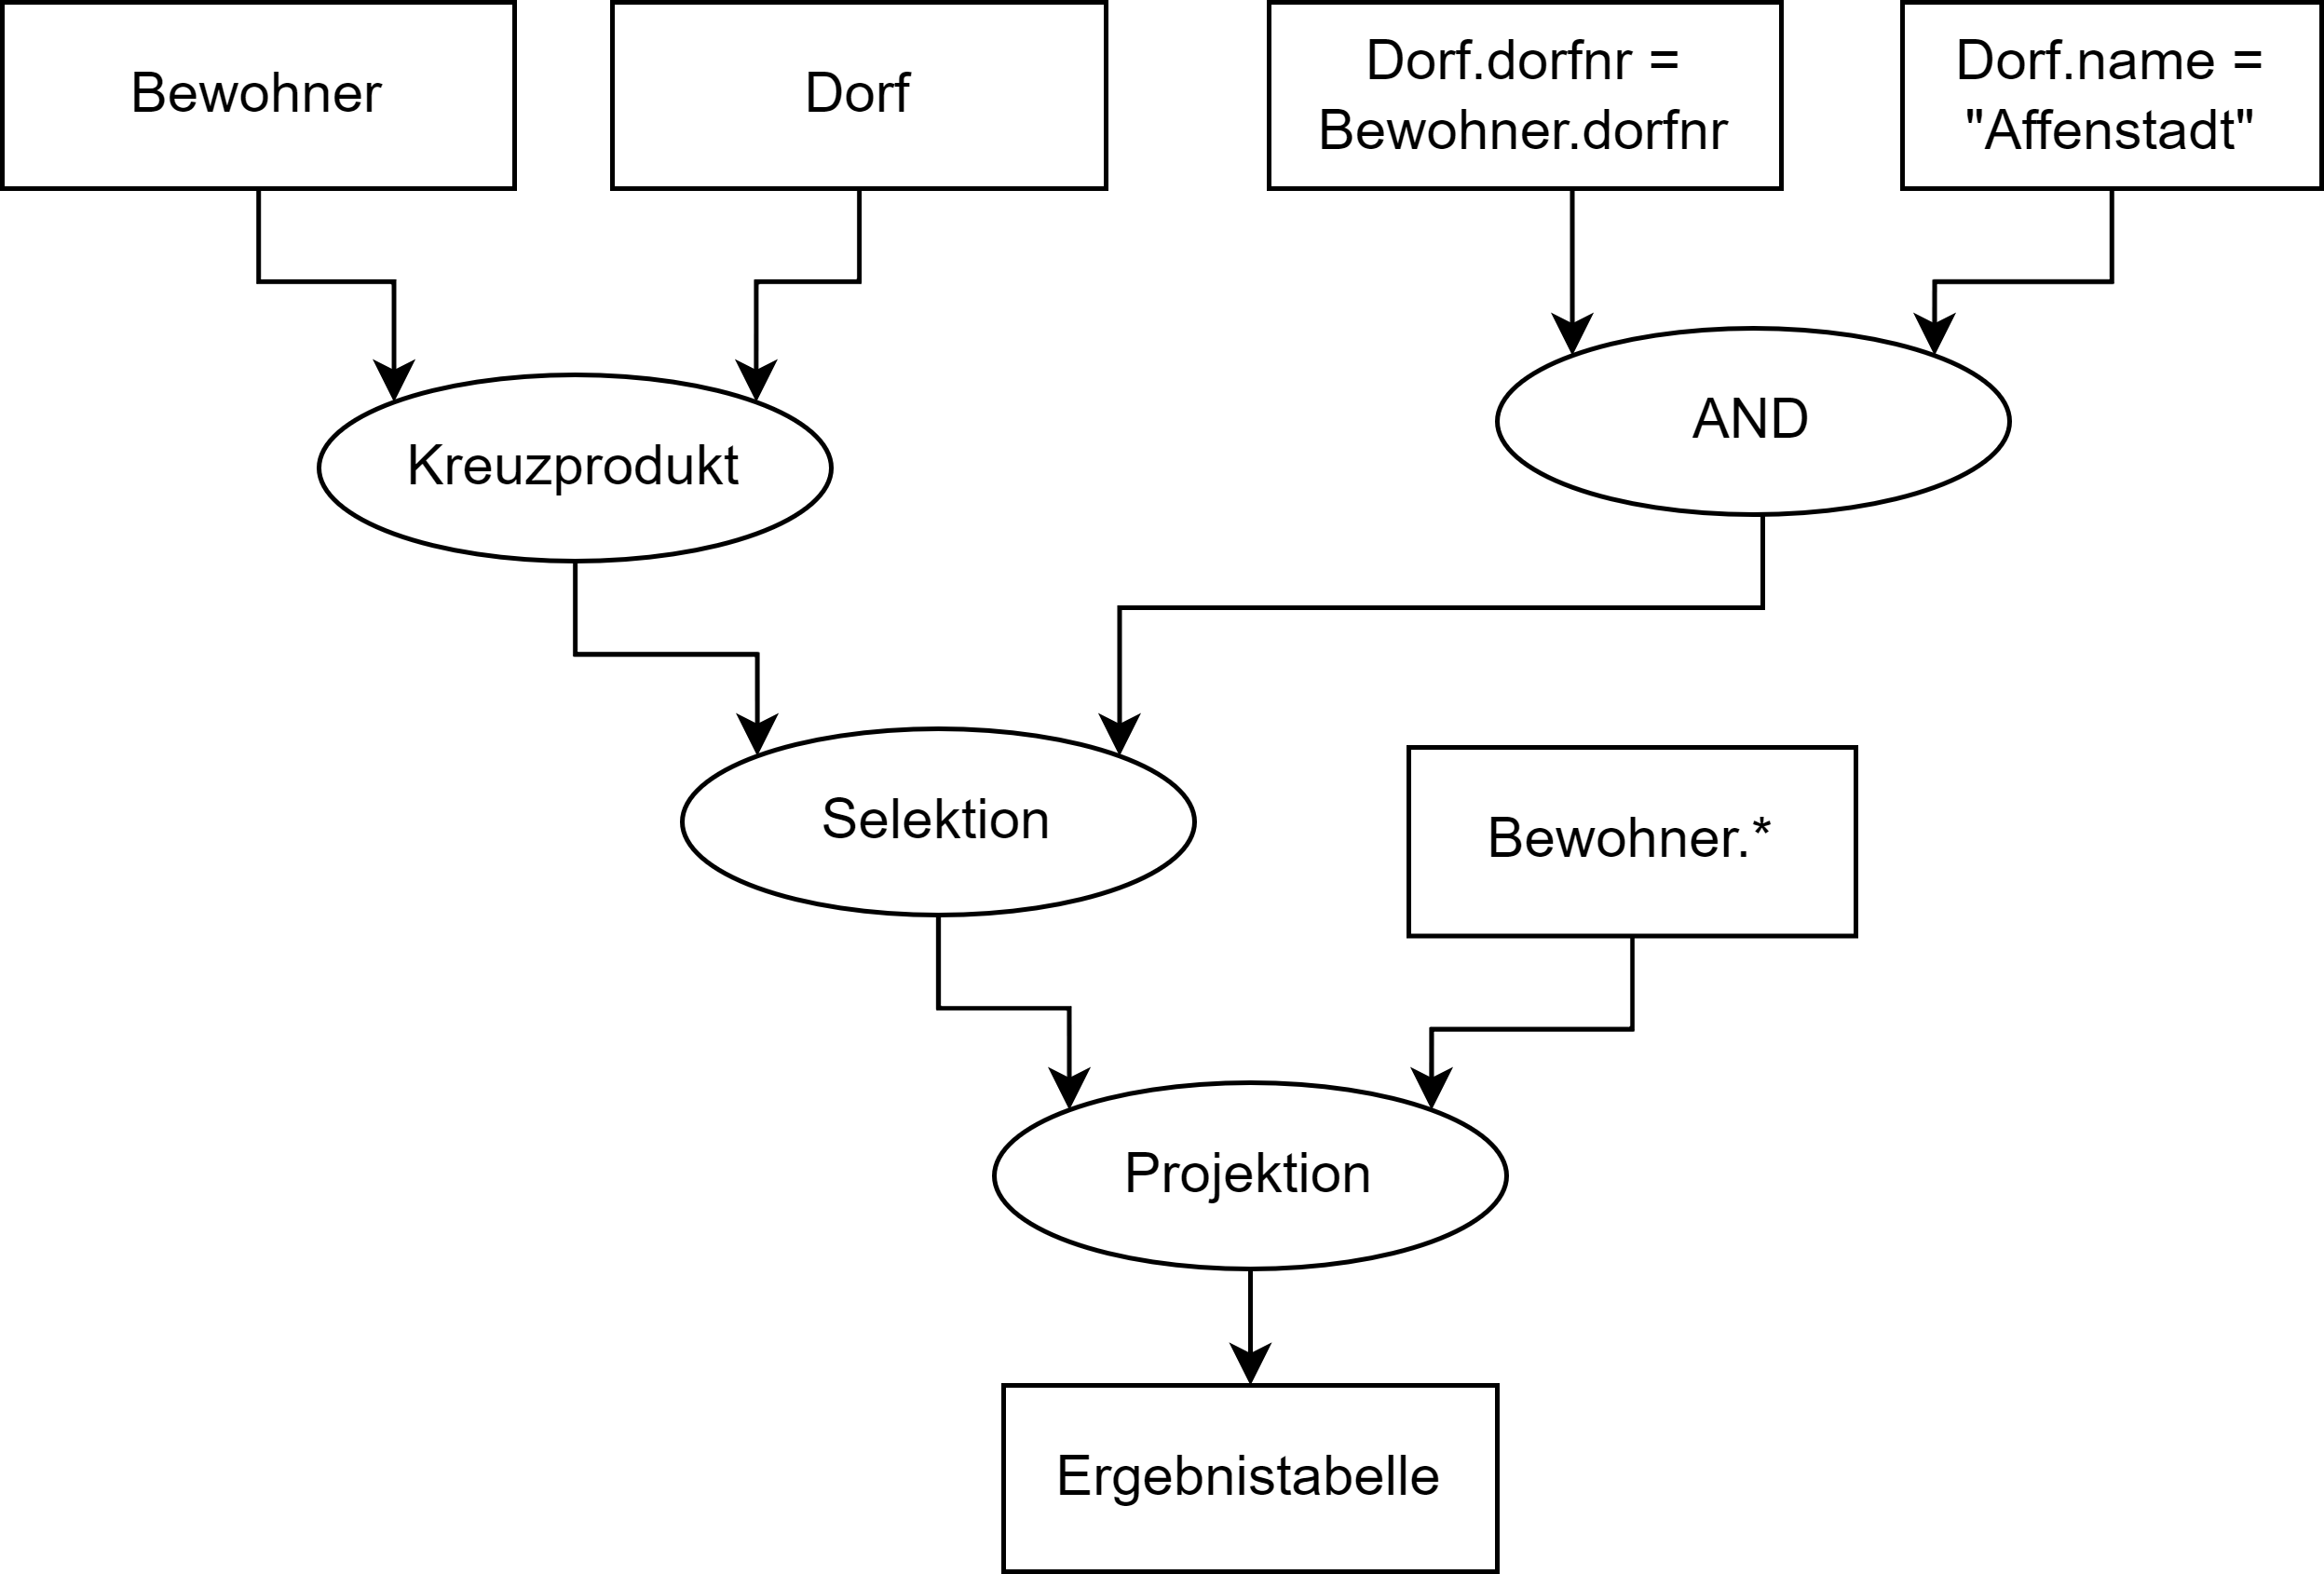
\includegraphics[width=0.8\textwidth]{Aufgaben/SQL-DFD_Uebung_img/4.png}}{20}

    \LoesungLine{SELECT Bewohner.* \\FROM Bewohner,Dorf \\ WHERE Bewohner.dorfnr=Dorf.dorfnr \\ AND Dorf.name = "Affenstadt"}{3}
